% LinuxPulse Beamer presentation. Compile from the repository root:
%   pdflatex -output-directory=docs docs/presentation.tex   (run twice for the outline)
\documentclass[aspectratio=169,10pt]{beamer}
\usetheme{metropolis}
\usepackage[T1]{fontenc}
\usepackage{lmodern,booktabs,graphicx}
\graphicspath{{assets/screenshots/}}
\title{LinuxPulse}
\subtitle{Real-Time Linux System Monitoring \& Performance Analytics}
\author{LinuxPulse Team}
\institute{Indian Institute of Technology Dharwad}
\date{}
\setbeamertemplate{navigation symbols}{}

\begin{document}
\maketitle

\begin{frame}{Problem statement}
\begin{itemize}
  \item \texttt{top} shows the present moment: no history, no statistics, no alerts.
  \item Goal: one desktop dashboard for CPU, RAM, swap, load and processes, with trends and thresholds.
  \item Constraint: small, modular, testable, built for Arch Linux / Omarchy.
\end{itemize}
\end{frame}

\begin{frame}{Objectives}
\begin{enumerate}
  \item Near-real-time CPU, memory, swap, load and process data (2\,s default).
  \item Bounded history (300 samples) and NumPy-ready statistics.
  \item Matplotlib charts embedded in Tkinter.
  \item Threshold alerts: CPU 80\,\%, RAM 85\,\%, swap 80\,\%.
  \item Mock mode that is always labelled and never mixed with live data.
  \item Profiling with GCC and gprof; automated build and tests.
\end{enumerate}
\end{frame}

\begin{frame}{Technology stack}
\begin{tabular}{ll}
\toprule Layer & Technology \\ \midrule
Data acquisition & \texttt{/proc}, Linux \texttt{top} via \texttt{subprocess} \\
GUI \& charts & Tkinter / ttk, Matplotlib (\texttt{FigureCanvasTkAgg}) \\
Analytics & Python, NumPy \\
Concurrency & \texttt{threading}, \texttt{queue} \\
Profiling & C++, GCC \texttt{-pg}, GNU gprof \\
Automation & GNU Make, Bash, \texttt{unittest}, Git \\ \bottomrule
\end{tabular}
\end{frame}

\begin{frame}[fragile]{System architecture}
\small
\begin{verbatim}
collector (M1)  -> dict, KiB
   | validate + to_snapshot()        main.py adapters (M5)
models.SystemSnapshot, bytes
   | AnalyticsEngine.add_snapshot()  (M2)
   | to_view_state()                 main.py adapters (M5)
queue.Queue(maxsize=256, drop-oldest)
   | root.after() polling, GUI thread only
Dashboard (M3) -> charts (M4)
\end{verbatim}
\normalsize
One background thread collects; the Tk main thread only drains the queue. \texttt{models.py} is the single data contract.
\end{frame}

\begin{frame}{Real-time monitoring}
\begin{columns}
\column{0.42\textwidth}
\begin{itemize}
  \item One \texttt{top} call per sample; CPU \% from \texttt{/proc/stat} deltas.
  \item GUI never blocks on collection.
  \item Newest state wins: full queue drops the oldest.
  \item Measured: 1 worker thread, queue size 0--1, clean shutdown.
\end{itemize}
\column{0.58\textwidth}
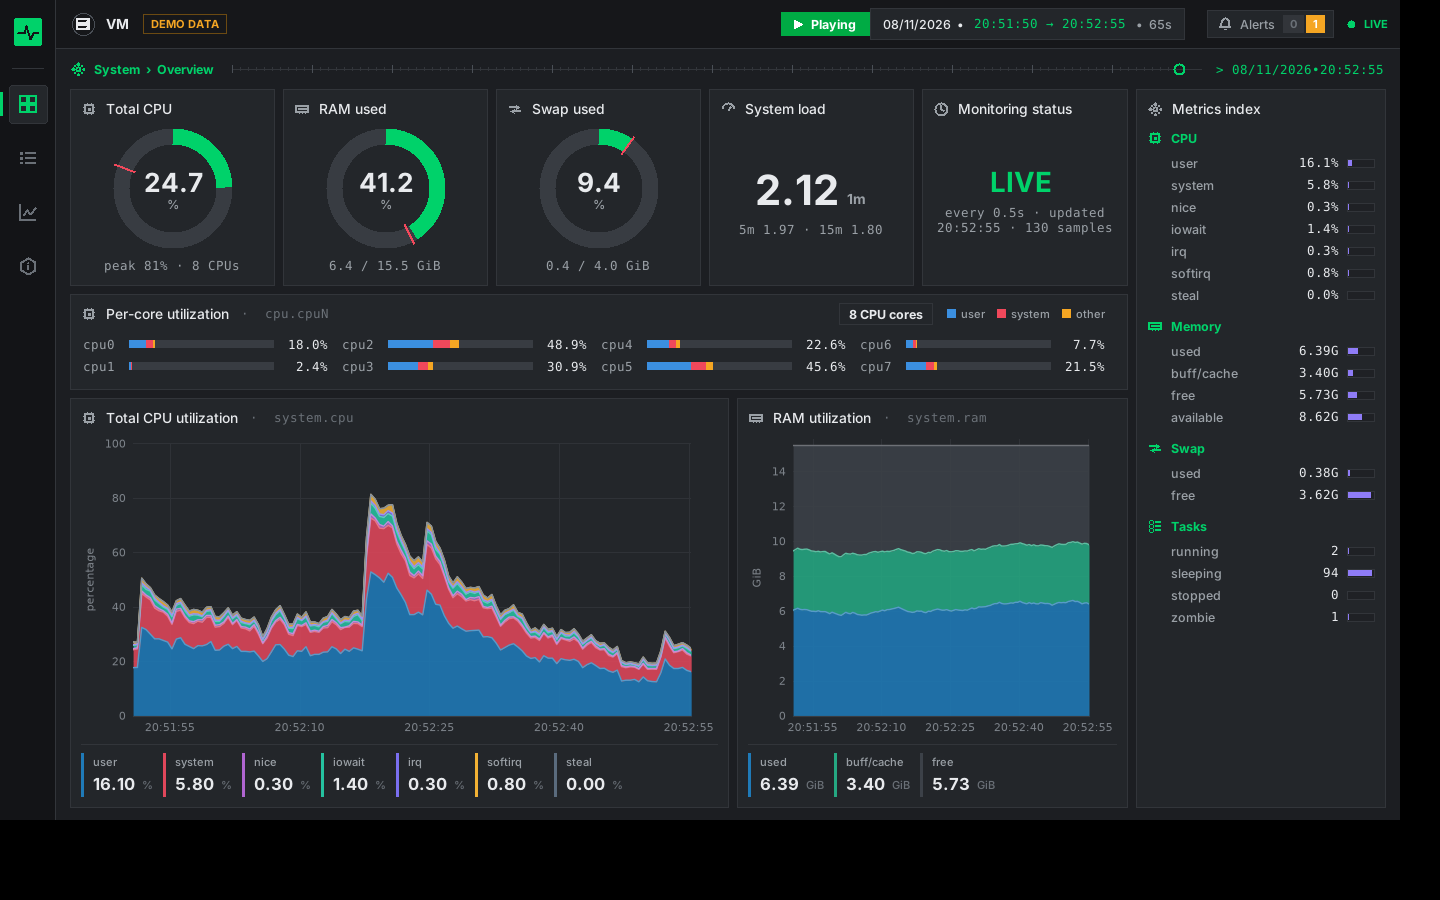
\includegraphics[width=\textwidth]{overview.png}
\end{columns}
\end{frame}

\begin{frame}{Analytics and visualization}
\begin{columns}
\column{0.42\textwidth}
\begin{itemize}
  \item Mean, peak, minimum, deviation, rolling values.
  \item Top CPU and memory processes.
  \item Alerts reach the top-bar badge and the alert list.
  \item Process table: sort, filter, search.
\end{itemize}
\column{0.58\textwidth}
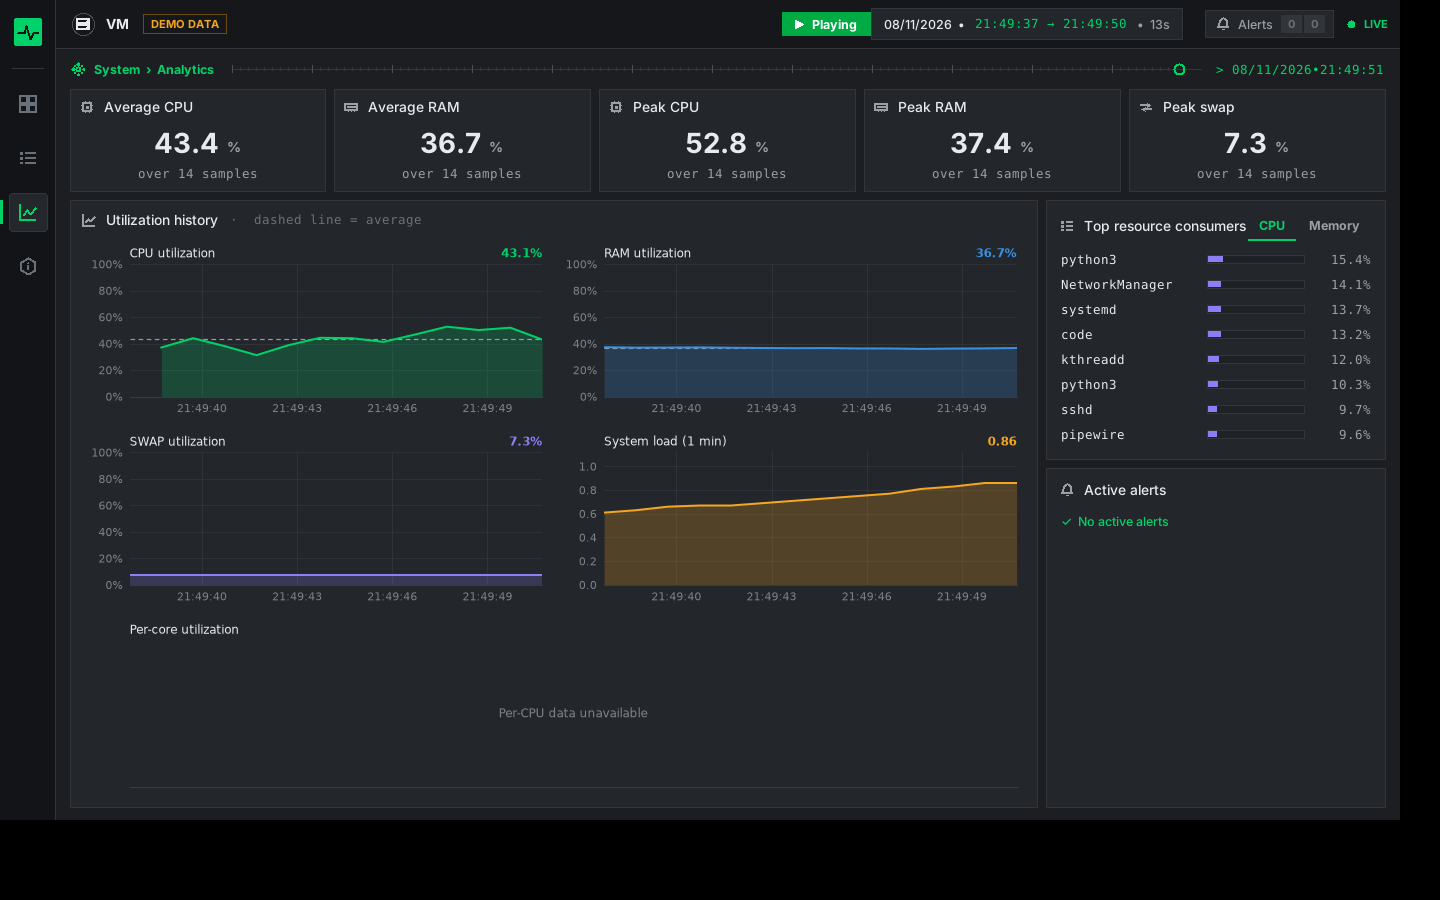
\includegraphics[width=\textwidth]{analytics.png}
\end{columns}
\end{frame}

\begin{frame}{Integration audit}
\begin{itemize}
  \item Teammate modules matched the contract; interfaces checked at start-up.
  \item Fixed: CPU alert default 90\,\% $\to$ 80\,\%; \texttt{top}'s truncated user names (\texttt{systemd+}) resolved in an adapter.
  \item Reported to owners: no per-core CPU, alerts always ``critical'', chart layout cost.
  \item Cost of LinuxPulse itself (default 2\,s): about 17\,\% of one core, 117--120\,MB, flat over a 190\,s run.
\end{itemize}
\end{frame}

\begin{frame}{Performance profiling (C++ benchmark, not the Python app)}
\begin{itemize}
  \item Workloads: large-array statistics, rolling average, process ranking, aggregation; deterministic.
  \item gprof call graph: \texttt{top\_processes} = 43.7\,\% of sampled time.
  \item Cause: copy 250 structs and fully sort to keep 5.
  \item Fix: \texttt{std::partial\_sort} on indices.
\end{itemize}
\medskip
\begin{tabular}{lrrr}
\toprule & Baseline & Optimized & Speedup \\ \midrule
Ranking only & 0.843\,s & 0.042\,s & 20.1$\times$ \\
Whole program & 1.424\,s & 0.603\,s & 2.36$\times$ \\ \bottomrule
\end{tabular}

{\footnotesize Median of 5 runs, \texttt{-O0}, one machine; identical output checksums.}
\end{frame}

\begin{frame}{Testing}
\begin{itemize}
  \item 120 \texttt{unittest} tests, all passing: parser, collector, analytics, visualization, controller, integration.
  \item GUI-level tests drive the real window: alerts, process table, main-thread-only drawing, shutdown, queue bound.
  \item Clean-checkout run: \texttt{make install}, \texttt{check}, \texttt{test}, \texttt{mock}, \texttt{run}, \texttt{profile}.
\end{itemize}
\end{frame}

\begin{frame}{Conclusion and future work}
\textbf{Delivered:} modular dashboard, mock and live modes, tests, build automation, measured optimization experiment.
\medskip

\textbf{Next:}
\begin{itemize}
  \item Per-core CPU in the collector; warning vs.\ critical alert levels.
  \item Cheaper chart redraws (freeze layout after first draw).
  \item \texttt{scripts/launch.sh}; macOS testing.
\end{itemize}
\end{frame}
\end{document}
